\subsection{Lightweight Authenticated Encryption With Associated Data }


Lightweight Authenticated Encryption with Associated Data (AEAD) algorithms are designed to efficiently provide both confidentiality and message integrity in a single operation. These algorithms offer a balance between security and performance, making them suitable for securing data both at rest and in motion \cite{el-hajj_analysis_2023}. The confidentiality aspect is achieved through the generated cipher, while authentication or message integrity is ensured through the tag generated during encryption. Upon receipt, the receiver can decrypt the cipher to access the original message and simultaneously verify the tag to ensure that neither the message nor the cipher has been altered during transmission.

\subsubsection*{AES-GCM}

AES-GCM is a family of authenticated encryption with associated data based on AES (Advanced Encryption Standard) and GCM (Galois Counter Mode). It was first presented by David A. McGrew and John Viega \cite{mcgrew_galoiscounter_nodate} in 2005. Since then it has been adopted for various applications including for TLS and IPSec implementation \cite{salowey_aes_2008}.  


\subsubsection*{ASCON}

ASCON is an authenticated encryption algorithm designed and developed by Christoph Dobraunig, Maria Eichlseder, Florian Mendel and Martin Schläffer \cite{dobraunigAsconV1Lightweight2021}. It become very popular after it wins the CASEAR NIST computation. The authors claim the main goal of the algorithm is to provide simplicity, online, security, side-channel robustness, single-pass and lightweight cipher for the resource-constrained device \cite{dobraunigAsconV1Lightweight2021}. It is also a well-performing algorithm for short messages \cite{dobraunigAsconV1Lightweight2021} like for applications to collect environment and operating conditions in industry 4.0

The algorithm can also be used on high-performing machines to provide encryption and decryption for time-critical applications. It can provide 128-bit key security \cite{dobraunigAsconV1Lightweight2021}, surpassing the currently accepted 80-bit security standard.


\begin{figure}[H]
    \centering
    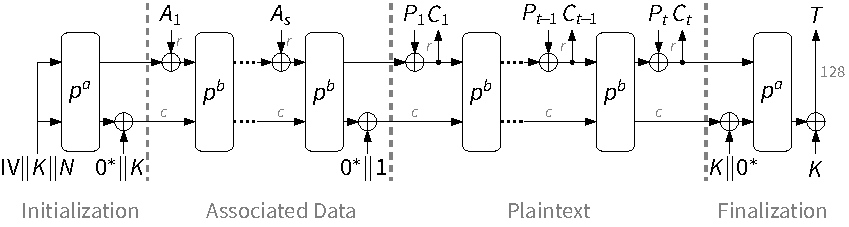
\includegraphics{images/fp/aead_encrypt.pdf}
    \caption{ASCON Encryption Mode of Operation (taken from \cite{dobraunig_ascon_nodate})}
    \label{fig:ascon-enc}
\end{figure}

The encryption and decryption process of ASCON is split into 4 main phases as depicted in Figure \ref{fig:ascon-enc} and \ref{fig:ascon-dec}. These are initialization, associated data processing, plain text/cipher text processing (depending on whether it is in encryption or decryption mod) and finalization. 



\begin{figure}[H]
    \centering
    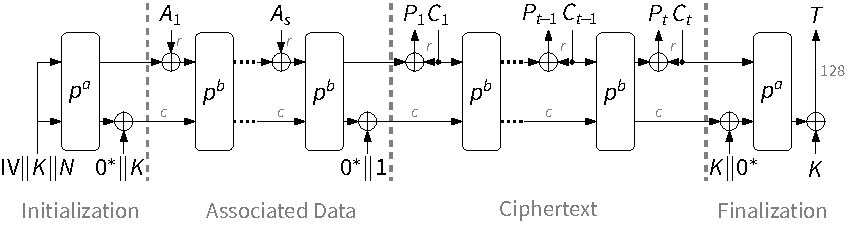
\includegraphics{images/fp/aead_decrypt.pdf}
    \caption{ASCON Decryption Mode of Operation (taken from \cite{dobraunig_ascon_nodate})}
    \label{fig:ascon-dec}
\end{figure}
